\documentclass[journal=esthag,manuscript=article]{achemso}
%%%%%%%%%%%%%%%%%%%%%%%%%%%%%%%%%%%%%%%%%%%%%%%%%%%%%%%%%%%%%%%%%%%%%
%% Place any additional packages needed here.  Only include packages
%% which are essential, to avoid problems later. Do NOT use any
%% packages which require e-TeX (for example etoolbox): the e-TeX
%% extensions are not currently available on the ACS conversion
%% servers.
%%%%%%%%%%%%%%%%%%%%%%%%%%%%%%%%%%%%%%%%%%%%%%%%%%%%%%%%%%%%%%%%%%%%%
\usepackage[T1]{fontenc}       % Use modern font encodings
\usepackage[utf8]{inputenc}
\usepackage{todonotes}
\usepackage{amsmath}

%%%%%%%%%%%%%%%%%%%%%%%%%%%%%%%%%%%%%%%%%%%%%%%%%%%%%%%%%%%%%%%%%%%%%
%% If issues arise when submitting your manuscript, you may want to
%% un-comment the next line.  This provides information on the
%% version of every file you have used.
%%%%%%%%%%%%%%%%%%%%%%%%%%%%%%%%%%%%%%%%%%%%%%%%%%%%%%%%%%%%%%%%%%%%%
%%\listfiles

%%%%%%%%%%%%%%%%%%%%%%%%%%%%%%%%%%%%%%%%%%%%%%%%%%%%%%%%%%%%%%%%%%%%%
%% Place any additional macros here.  Please use \newcommand* where
%% possible, and avoid layout-changing macros (which are not used
%% when typesetting).
%%%%%%%%%%%%%%%%%%%%%%%%%%%%%%%%%%%%%%%%%%%%%%%%%%%%%%%%%%%%%%%%%%%%%
\newcommand*\mycommand[1]{\texttt{\emph{#1}}}


%%%%%%%%%%%%%%%%%%%%%%%%%%%%%%%%%%%%%%%%%%%%%%%%%%%%%%%%%%%%%%%%%%%%%
\author{Eduard Szöcs}
\affiliation[Institute for Environmental Sciences]{Institute for Environmental Sciences, University of Koblenz-Landau, Germany}
\email{szoecs@uni-landau.de}
\phone{+49 (0)6341 280 31552}

\author{Marvin Brinke}
\affiliation[German Federal Institute of Hydrology]{German Federal Institute of Hydrology (BfG), Koblenz, Germany}

\author{Bilgin Karaoglan}
\affiliation[German Federal Environmental Agency]{Federal Environmental Agency (UBA), Dessau-Roßlau, Germany}

\author{Ralf B. Schäfer}
\affiliation[University Koblenz-Landau]{Institute for Environmental Sciences, University of Koblenz-Landau, Germany}


%%%%%%%%%%%%%%%%%%%%%%%%%%%%%%%%%%%%%%%%%%%%%%%%%%%%%%%%%%%%%%%%%%%%%
\title[Pesticides small streams]{Pesticides in small agricultural streams in Germany}
\abbreviations{mo, pest, ger, tu}
\keywords{Monitoring, Neonicotinoid, Germany, Toxic Units, Freshwater}
% RAC, 

%%%%%%%%%%%%%%%%%%%%%%%%%%%%%%%%%%%%%%%%%%%%%%%%%%%%%%%%%%%%%%%%%%%%%
\begin{document}
%%%%%%%%%%%%%%%%%%%%%%%%%%%%%%%%%%%%%%%%%%%%%%%%%%%%%%%%%%%%%%%%%%%%%
%% The "tocentry" environment can be used to create an entry for the
%% graphical table of contents. It is given here as some journals
%% require that it is printed as part of the abstract page. It will
%% be automatically moved as appropriate.
%%%%%%%%%%%%%%%%%%%%%%%%%%%%%%%%%%%%%%%%%%%%%%%%%%%%%%%%%%%%%%%%%%%%%
\begin{tocentry}

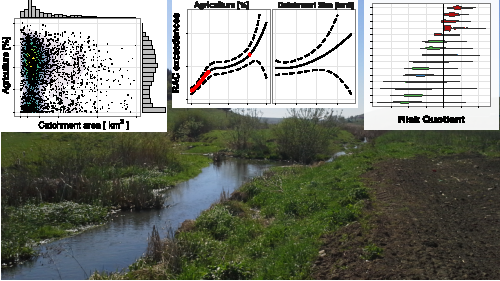
\includegraphics[width=0.7\textwidth]{abstract.pdf}

\end{tocentry}



%%%%%%%%%%%%%%%%%%%%%%%%%%%%%%%%%%%%%%%%%%%%%%%%%%%%%%%%%%%%%%%%%%%%%
\begin{abstract}
Fehlt noch...
\end{abstract}


%%%%%%%%%%%%%%%%%%%%%%%%%%%%%%%%%%%%%%%%%%%%%%%%%%%%%%%%%%%%%%%%%%%%%
\section{Introduction}

More than 50\% of the total land area in Germany are used by agriculture \citep{statistisches_bundesamt_bodenflache_2014}.
In the year 2014 more the 45,000 tonnes of 766 authorized pesticides were sold for application on this area \citep{bundesamt_fur_verbraucherschutz_und_lebensmittelsicherheit_absatz_2015}.
The applied pesticides may enter surface waters via spray-drift, edge-off-field run-off or drainage, with run-off being one of the major input routes \citep{schulz_comparison_2001,liess_determination_1999}.
Once entered the surface waters pesticides are frequently detected in environmental monitoring \citep{malaj_organic_2014} and may have adverse effects on biota and ecosystem functioning \citep{schulz_field_2004, schafer_effects_2007}.

\citet{malaj_organic_2014} analysed data supplied to the European Union (EU) in the context of the Water Framework Directive (WFD) and showed that pesticides jeopardize the health of freshwater ecosystems.
However, this study reflected only a small part of data that is available from national monitoring programs.
These programs are setup for determination and surveillance of the chemical and ecological status of surface, ground and drinking water.
Large amounts of data are generated, which possibly can also be used to answer other questions.
In Germany monitoring programs are setup independently by the federal states in compliance with the WFD \citep{quevauviller_water_2008} and additional state specific needs.
However, currently there is no curated national-wide compilation of this data available.

\citet{stehle_pesticide_2015} compiled 1566 measured concentrations of 23 insecticides in the EU from scientific publications. 
They found that insecticides that many of these measurements exceed regulatory acceptable concentrations (RAC), especially in very small catchments \textless $1~km^2$.
Small water bodies are important refuges of biodiversity \citep{davies_comparison_2008} and enable downstream colonisation of polluted streams \citep{liess_analyzing_2005}.
At the same time they may be exposed to a high risk of pesticide contamination from adjacent agricultural areas and low dilution effects \citep{liess_determination_1999}.
Although small streams comprise a major fraction of streams \citep{nadeau_hydrological_2007}, relatively little is know about their chemical and ecological status.

The aim of this study was to compile all available chemical monitoring data in Germany and to answer the questions: \\
(i) Can the currently available monitoring data used for a representative description of the pollution situation? \\
(ii) Are small agricultural waters more polluted compared to bigger streams? Are there thresholds in these relationships? \\
(iii) How polluted are small streams and which pesticides are most important?


\section{Methods}
\subsection{Data compilation}

We queried chemical monitoring data of pesticides from sampling sites with catchment sizes $\mathrm{< 100km^2}$ for the years 2005 to 2015 from all 13 non-city federal states of Germany.
Additionally, we compiled data available from previous studies and searched online databases.
This yielded to a total of more then 30 datasets of different formats.
In the following we will use the ISO 3166-2:DE standard abbreviations for federal states.

We homogenized and unified these datasets into a common database.
We implemented a robust and reproducible data cleaning work flow \citep{poisot_best_2015}, though parts of the dataset are proprietary.
An overview of the data cleaning process is provided in the supplemental materials.  
To assess whether samples were taken during potential rainfall events we performed spatio-temporal intersection of sampling events with daily precipitation data from the sampling date and the day before. \citep{rauthe_central_2013}.

\subsection{Characterization of chemical pollution}
We characterized chemical pollution (excluding sum parameters) using three indicators:

\begin{enumerate}
  \item National and international Environmental Quality Standards (EQS) \citep{ogewv_verordnung_2011,european_union_directive_2013}:
  We used only Maximum Annual Concentration EQS (MAC-EQS) for characterization.
  These were available for 29 compounds (Supplement, Table xxx\todo{ref}).

  \item Regulatory Acceptable Concentrations (RAC) \citep{brock_linking_2010}:
  This is the lowest concentration at which no acceptable biological effects are expected. 
  These are derived during authorization process of pesticides and incorporate also an uncertainty factor.
  The German Federal Environmental Agency provided RACs for 105 compounds (Supplement, Table xxx\todo{ref}).  
  We expressed RAC as Risk Quotient (RQ):
  \begin{equation}
  RQ_i = \frac{C_i}{RAC_i}
  \end{equation}
  Where $C_i$ is the concentration of a compound $i$ bin a sample.

  \item Maximum Toxic Units ($\mathrm{TU_{max}}$)  \citep{sprague_measurement_1970}: 
  \begin{equation}
  TU_{max} = max(\frac{C_i}{EC_{50, D.magna, i}})
  \end{equation}

  Where $C_i$ is the concentration of compound $i$ in a sample and $EC_{50, D.magna, i}$ is the concentration of this compound where 50\% of the exposed animals showed after 48 hours an effect in a laboratory study.
  We compiled $EC_{50, D.magna}$ values from literature \citep{malaj_organic_2014}, databases \citep{lewis_international_2016,u.s._epa_ecotoxicology_2015} or model predictions \citep{schuurmann_quantitative_2011}, where experimental data had priority.
  We could compile $EC_{50, D.magna}$ values for 394 compounds (Supplement, Table xxx\todo{ref})).
  We used the maximum TU per sample, as it is independent of the number of measured compounds and makes no assumptions on the mode of action.
  Additionally, we also calculated the sum of toxic units ($TU_{sum}$).
  A table of all included compounds can be found in the supplement.
\end{enumerate}


\subsection{Characterization of catchments}
We delineated catchments upstream of the sampling sites using a digital elevation model \citep{eea_digital_2013} and a multiple flow direction algorithm \citep{holmgren_multiple_1994} as implemented in GRASS GIS 7 \citep{neteler_grass_2012}.
Catchment delineation has been manually checked for accuracy. 
In areas with low relief energy the delineation algorithm did not produce accurate results and we used river catchments provided by federal state authorities in these cases.
For each catchment we calculated the relative coverage (\%) with agricultural areas based on Official Topographical Cartographic Information System (ATKIS) of the land survey authorities.


\subsection{Statistical analyses}

All data-processing and analyses have been performed using R \citep{r_core_team_r:_2016}.
To display differences in the spectra of analysed compounds between federal states we used Multidimensional Scaling (MDS) based on Jaccard dissimilarity in conjunction with hierarchical clustering using the vegan package \citep{oksanen_vegan:_2016}.
We expected non-linear responses to agriculture and catchment size and therefore, used generalized additive models (GAM) to identify relationships \citep{fewster_analysis_2000}.

We modeled the number of RAC exceedances as:

\begin{align}
\begin{split}
  No_i \sim NB(\mu_i, k) \\
  E(No_i) = \mu_i~and~Var(No_i) = \mu_i + \frac{\mu_i^2}{k} \\
  log(\mu_i)= \beta_0 + f_1(Agri_i) + f_2(Size_i) + log(n_i) \\
\end{split}
\end{align}

where $No_i$ is the observed number of exceedances at site $i$, $Agri_i$ the proportion of agriculture within the catchment and $Size_i$ the catchment size of the site. 
We modeled $No_i$ as resulting from a negative binomial distribution ($NB$) and used the number of sampling events per site ($n_i$) as an offset to account different sampling efforts. 
$f_1$ and $f_2$ are smoothing functions using thin plate regression splines \citep{wood_thin_2003}.
The degree of smoothness was estimated using restricted maximum likelihood (REML) during model fitting process \citep{wood_fast_2011}.
Similar models were fitted to the number of EQS-exceedances and the 95th percentile of $TU_{max}$ (see Supplement for details). 
We used pointwise 95\% Confidence Intervals of the first derivative of the fitted smooth to check if there are regions of statistically significant changes.
GAMs were fitted using the mgcv package \citep{wood_fast_2011}.


\section{Results}
\subsection{Overview and representativeness of compiled data}

The compiled dataset comprised only few standing waters (58 sites) and the majority (90\%) of samples where taken via grab sampling.  % see clean.R for numbers
Therefore, we report only results of grab samples from streams. 
The analysed dataset comprised 2,918,604 measurements from 42,236 samples from 3,049 sampling sites.  %see do_overview.R for numbers.
We found big differences in the number of sampling sites between federal states (Figure \ref{fig:fig1} and Supplement, Table \todo{Set ref to table}).

\begin{figure}[ht]
  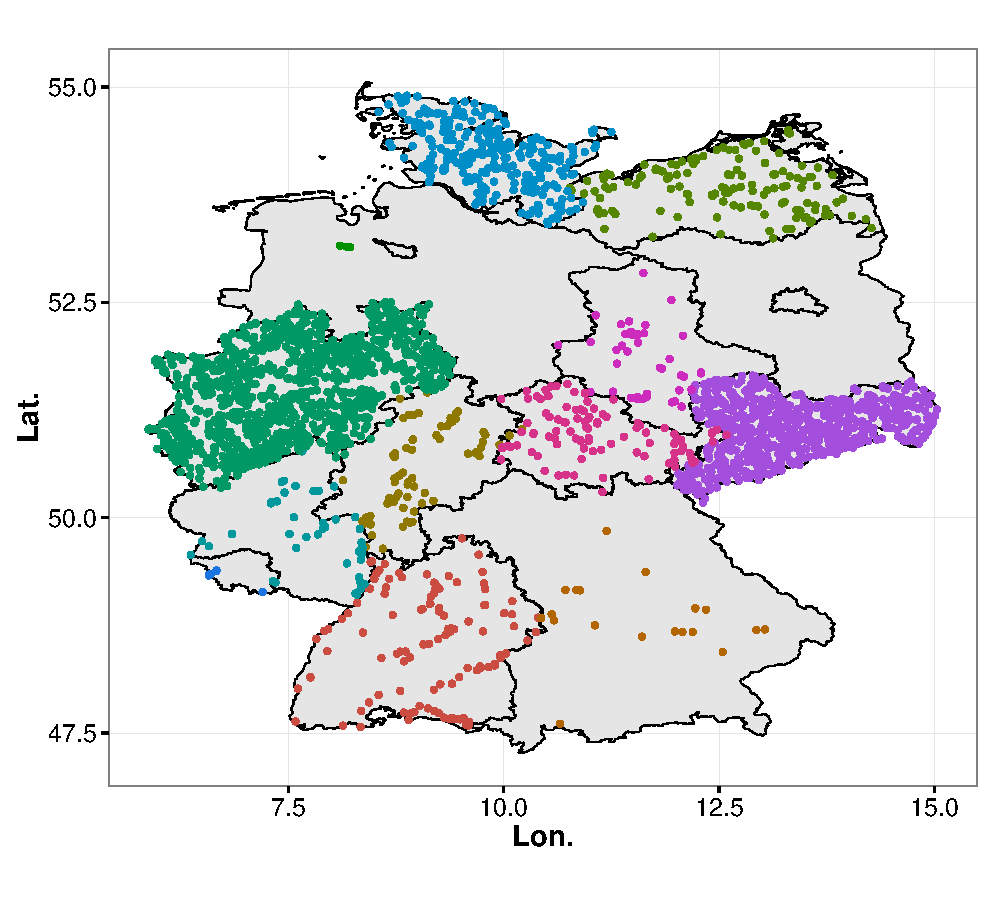
\includegraphics[width=0.6\textwidth]{figure1.pdf}
  \caption{Spatial distribution of the 3109 sampling sites. Colour codes different federal states.}
  \label{fig:fig1}
\end{figure}

In total 484 different compounds used as pesticides and their metobalites were measured at least once (Supplement, Table \todo{Set ref to table}). 
Most of the compounds were herbicides (179), followed by insecticides (117) and fungicides (109).
We found substantial differences of the spectra of analysed compounds between federal states (Figure \ref{fig:fig2}).
Hierarchical clustering revealed three groups:
i) with less then 100 compounds (SL, ST and TH), \\
ii) with a medium sized spectra and \\
iii) with a big and distinct spectra (RP and NI).

Only 5.5\% (160,800) of all measurements were detects above the limit of quantification (LOQ).
The spatio-temporal intersection revealed that 5\% of the samples were taken at or after days with rainfall events greater than 10mm / day. \todo{ref supplement}.

\begin{figure}[ht]
  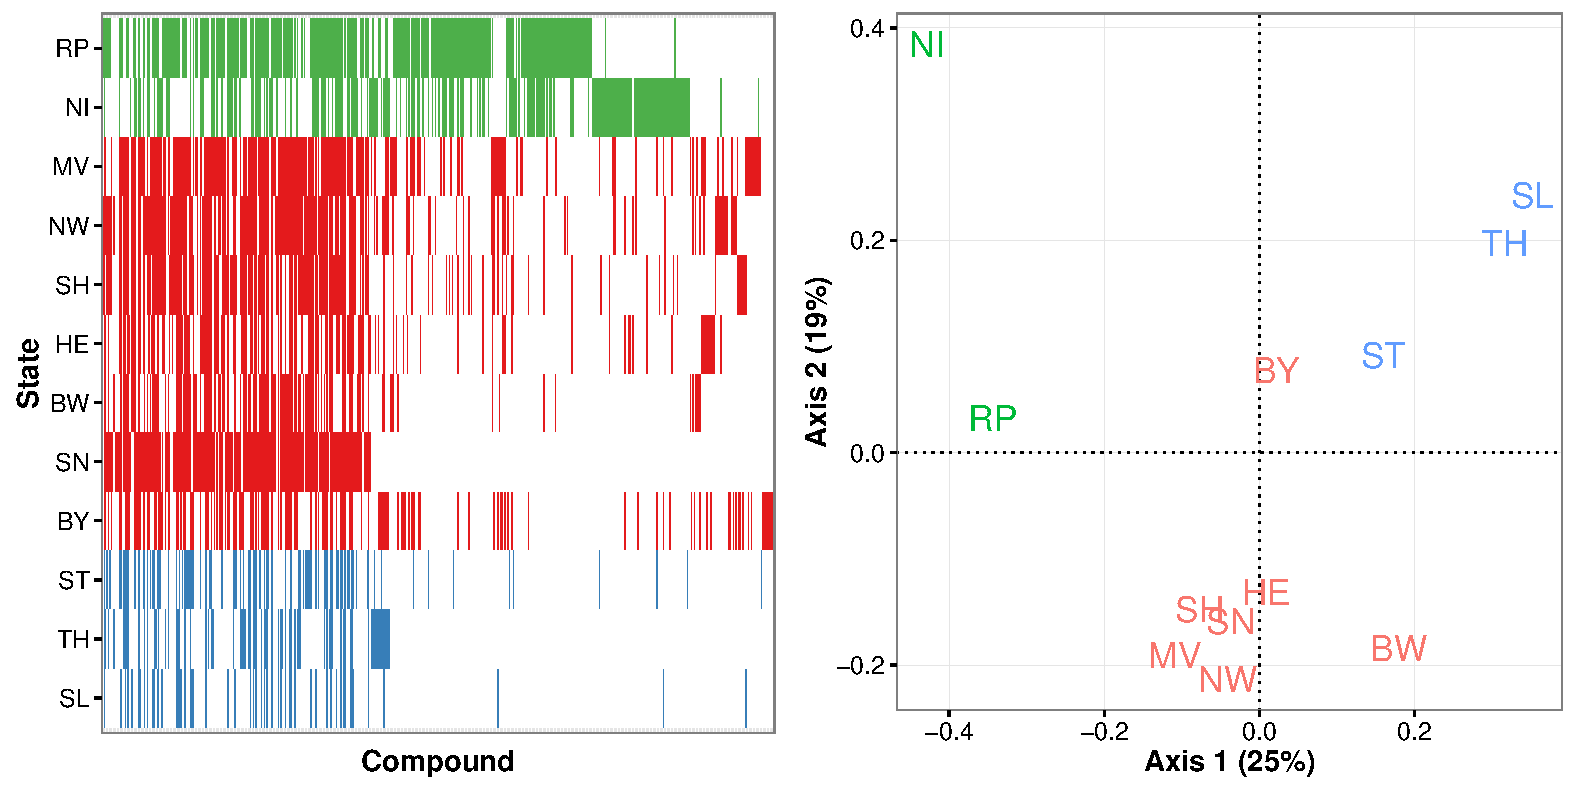
\includegraphics[width=\textwidth]{figure2.pdf}
  \caption{Compound spectra of the different federal states. Left: Barcode plot - Each vertical line is an analysed compound. Right: MDS ordination. 
  Colors according to three groups determined by hierarchical clustering (see Supplement Figure xxx).}
  \label{fig:fig2}
\end{figure}

We were able to derive for 2376 sites catchment sizes and the proportion of agriculture within catchments. 
The distribution of sampling sites across catchment area and agricultural area in the catchment revealed a sharp decline in the distribution of catchment-sizes below $10~km^2$, with most sampling sites with catchments between 10 and 25 $km^2$ (Figure \ref{fig:fig3}).
The proportion of agriculture in the catchments decreased with increasing catchment size.

\begin{figure}[ht]
  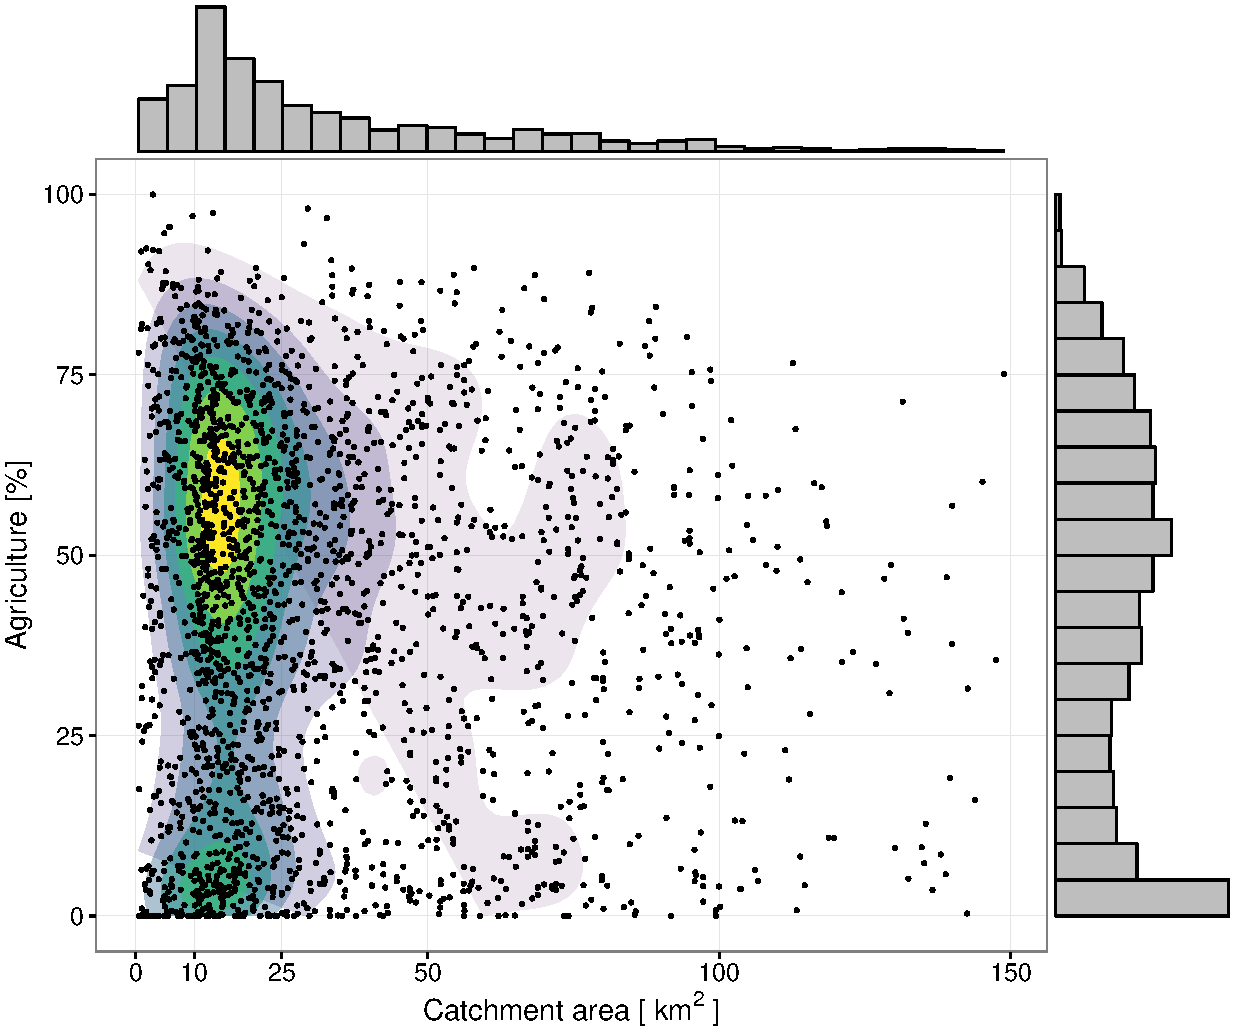
\includegraphics[width=.8\textwidth]{figure3.pdf}
  \caption{Distribution of catchment area and agriculture within the catchment area across the sampling sites.
  Only sampling sites with catchment area < 150 km\textsuperscript{2} are displayed. 
  Colour codes the 2-dimensional density of points.
  }
  \label{fig:fig3}
\end{figure}



\subsection{Are small agricultural waters more polluted compared to bigger streams?}

Modeling the number of RAC exceedances as function of agriculture within catchment and catchment size revealed that there is a strong and statistically significant increase up to 25\% agriculture.
Above this threshold the exceedances level off followed by a increase above 75\% (Figure \ref{fig:fig4}, left).

We could no detect any effect of catchment size on the number of RAC exceedances (Figure \ref{fig:fig4}, right) and no interaction between these two predictors.

\begin{figure}[ht]
  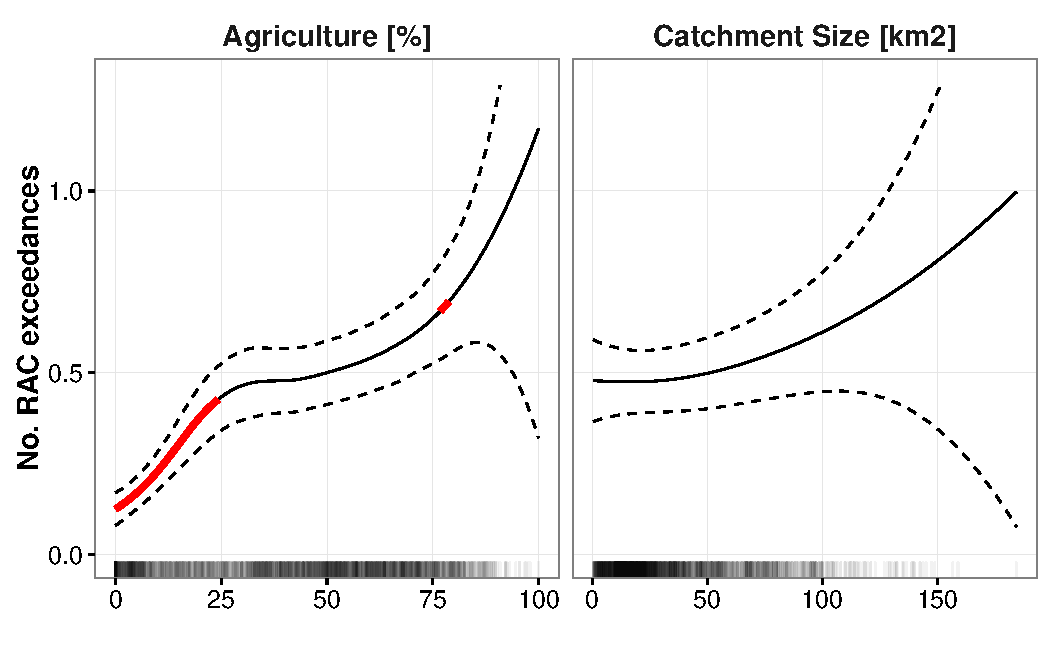
\includegraphics[width=0.95\textwidth]{figure4.pdf}
  \caption{Effect of agriculture within the catchment (left) and catchment size (right) on the number of RAC exceedances. Red line marks statistically significant changes. Dashed lines denote 95\% pointwise Confidence Intervals.
  }
  \label{fig:fig4}
\end{figure}

The number of EQS-exceedances and the 95th percentile of $TU_{max}$ showed similar patterns and thresholds (see Supplement Figure Sxxx - Sxxx). \todo{references}


\subsection{Pollution of small agricultural streams}
Based on the results previous results and given the low amount of sample sites with catchment sizes below 10 km\textsuperscript{2} we explored the pollution of small agricultural streams, defined as streams with catchment size less than 30 km\textsuperscript{2} and more than 25\% agriculture within the catchment (n = 1030 sites with 10591 samples and 36550 measurements).
%EQS
Out of the 29 compounds with EQS, the most frequent EQS exceedances were recorded for the herbicides Nicosulfuron (2.1\%, n = 1769), Flufenacet (1.1\%, n = 6301) and Isoproturon (0.7\%, n = 8380). 
Other compounds show exceedances only at less then 0.5\% of all samples (Figure \ref{fig:fig5}A).
% RAC
Neonicotinoid Insecticides and Chlropyrifos showed highest risk quotients.
For Thiacloprid, Imidacloprid and Chlorpyrifos RAC was less than LOQ, therefore, all detections have a RQ \textgreater 1 (Figure \ref{fig:fig5}B). 
In 15\% of all samples (n = 6377) risc quotients higher then 1 were observed.
Highest RQ were observed for Chlorpyrifos (244), Dimoxystrobin(117) and Isoproturon (80). 
% TU
In 33\% of the samples no pesticides were detected. 
The mean $log(TU_{max})$ for detects was -4.6.
2.6\% of the samples showed $log(TU_{max})$ values greater then -2 (Figure \ref{fig:fig5}C).
We found a high correlation of $log(TU_{max})$ and $TU_{sum}$ \todo{ausrechnen und r angeben}, with a maximum higher value of $TU_{sum}$ xx units.
%Mixtures
In most samples (55.5\%) more then one compound was detected, with a maximum of 54 different compounds (Figure \ref{fig:fig5}D). 

%% Add more numbers / percentages here => compare with knauer/stehle/Vijver

\begin{figure}[h]
  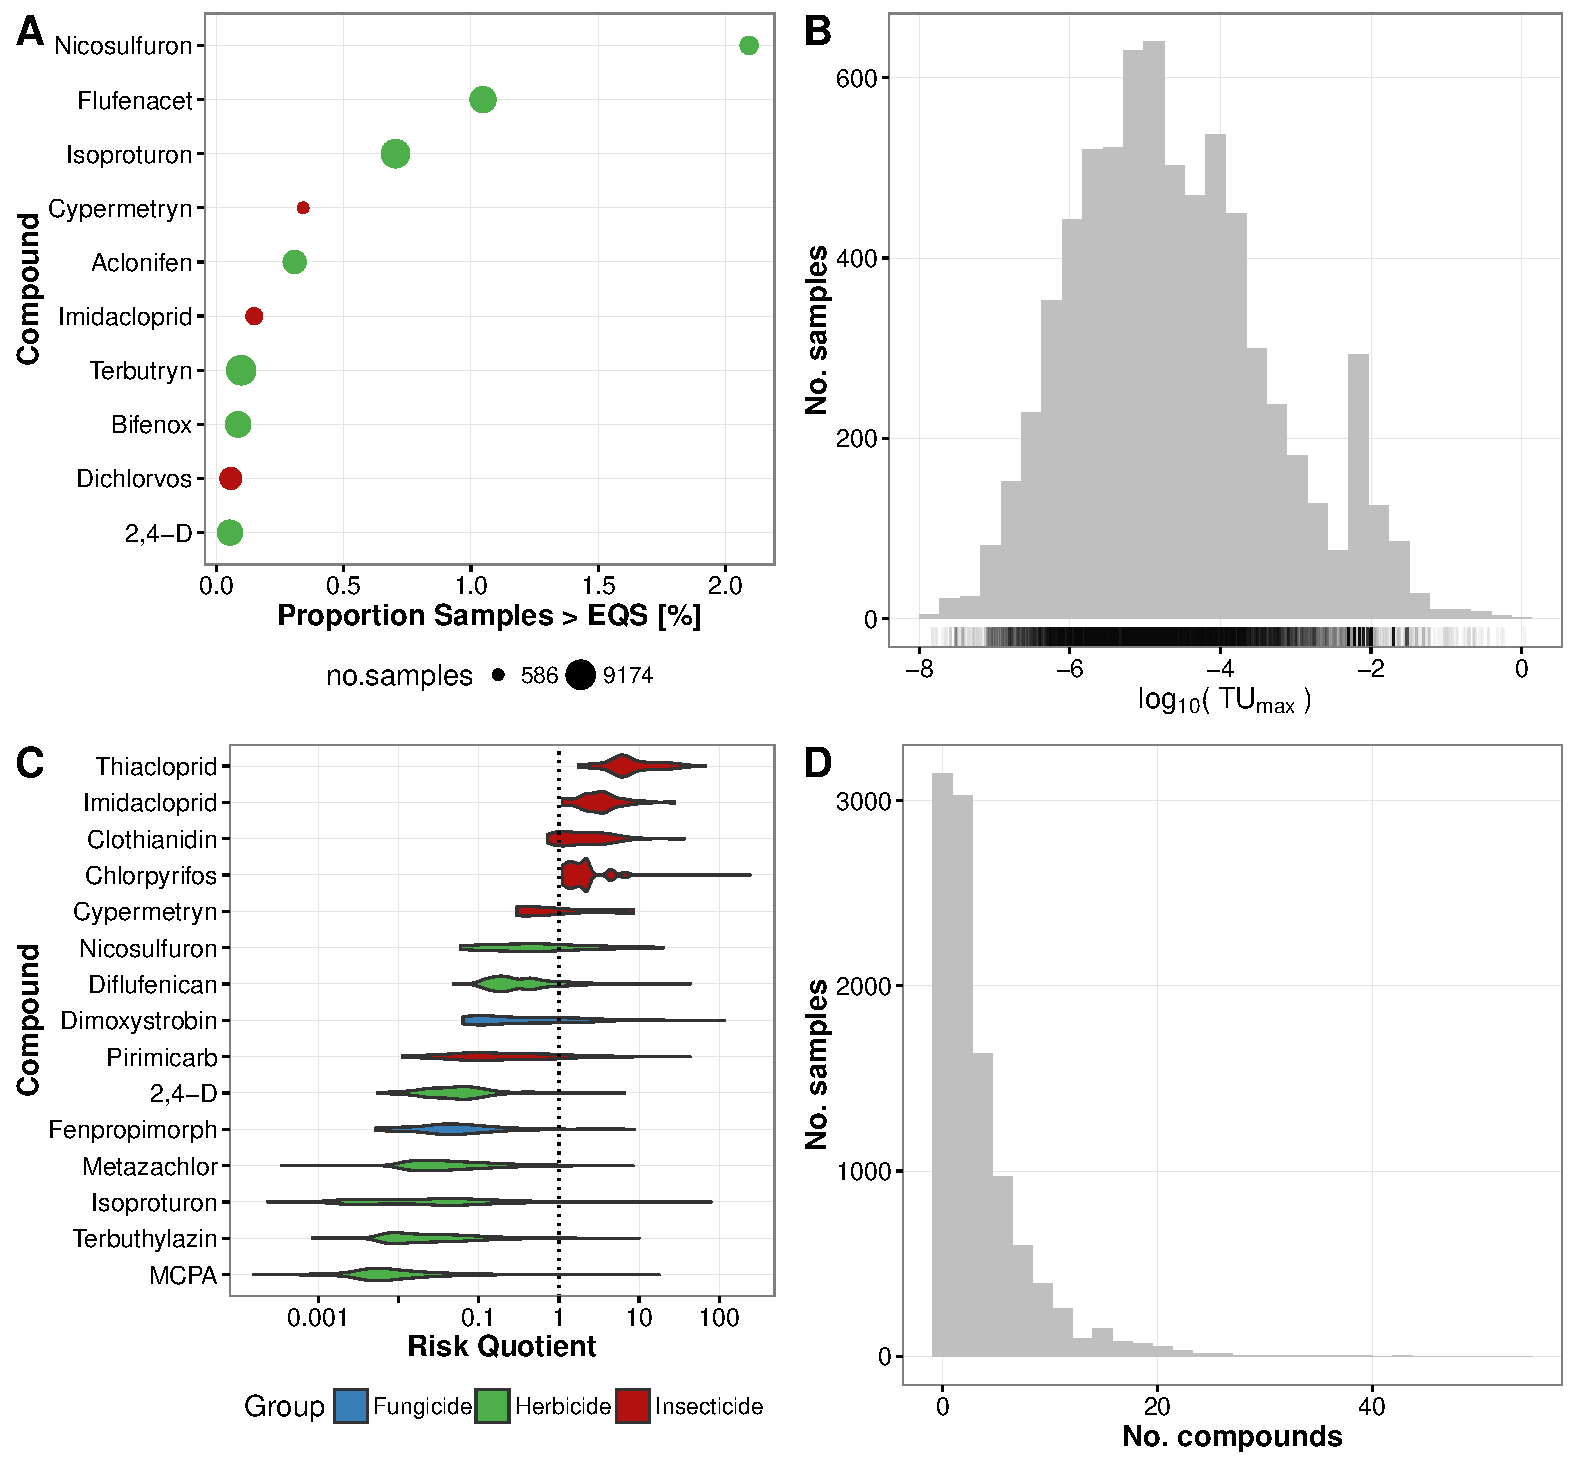
\includegraphics[width=0.9\textwidth]{figure5.pdf}
  \caption{Overview on pesticide pollution of small agricultural streams. 
      \textbf{A}: 10 compounds with most frequent EQS exceedances. See B for color legend.
      \textbf{B}: Distribution of $TU_{max}$ values. Values with $TU_{max} = 0$ are not displayed (3501 out of 10591 samples).
      \textbf{C}: 15 compounds with highest risk quotients.
      \textbf{D}: Distribution of the number of detected compounds in a sample.
  }
  \label{fig:fig5}
\end{figure}



\section{Discussion}

\subsection{Representativeness of the dataset}
The compiled dataset of governmental monitoring data represents currently the most comprehensive one available for Germany.
Similar nationwide datasets have been compiled for the Netherlands \citep{vijver_spatial_2008}, Switzerland \todo{cite munz} and the United States (Water Quality Portal (WQP) \url{www.waterqualitydata.us}).

\todo{compare numbers of different atlases, number of sites / compounds}.

Nevertheless such nationwide compilations, may not only be useful for governmental surveillance, but also to answer other questions, like validation of exposure modeling \todo{cite knäbel?}, retrospective evaluation of regulatory risk assessment \citep{knauer_pesticides_2016,stehle_pesticide_2015}, investigation of pesticide mixtures \todo{cite schreiner} or scientific research.

% current problems in monitoring and possible solutions
A nationwide assessment is hampered \todo{check verb} by the inhomogeneity of monitoring data between federal states:
There are not only big differences in the spatial distribution and quantity of sampling sites (Figure \ref{fig:fig1}), but also the spectrum of analysed compounds (Figure \ref{fig:fig2}) and differences in the quality of chemical analyses.
Future monitoring programs should aim at resolving these differences in order to enable a nationwide assessment. 



\subsection{Influence of catchment area and agriculture}
% agriculture
We found a strong influence of agriculture on the pollution of streams.
If there is more the 25\% agriculture within a catchment pesticides can be detected in streams and may have biological effects \todo{citation needed}.

% size
We did not find support for our hypothesis that small streams are more polluted then big streams, though previous studies have show such a relationship \citep{schulz_field_2004,stehle_pesticide_2015}.
This could be explained by the relatively small gradient of catchment sizes in our dataset, with most of the streams being \textless $100~km^2$ (Figure \ref{fig:fig3}, top).
For example the gradient of \citet{schulz_field_2004} covered 6 orders of magnitude.
Another reason might be the the unequal distribution of catchment sizes, with less sites \textless $10~km^2$ and \textgreater $100~km^2$(Figure \ref{fig:fig3}, top).







% Cite Schreiner in review
% combination with biological data.

% underestimation of grab sampling (Stehle et al. 2013). 

% Stehle nur insectizide
% malaj nur WFD?

% maxtu vs sumTU vs most sensitive => check publication.

% Stehle + Munz + Schulz kleine gewässer mehr belastet?
% Munz auch landwirtschaft

% kleinere prozent werte wegen saisonalität / Proben im winter






\subsection{Pollution of streams}

% EQS

% RAC
\citet{stehle_pesticide_2015} found the highest percentage of RAC exceedances organophosphate insecticides. 
Our results revealed that neonicotinoid insecticides show high exceedances, followed by the organophosphate chlorpyrifos. 
This difference can be attributed to the low sample size for neonicotinoid insecticides in their study (n = 33) compared to the dataset presented here \todo{zahlen neonics} and shows that this class may pose a high risk to freshwaters \todo{anderes Wort}.
Our results show lower proportions of exceedances compared to \citet{stehle_pesticide_2015}, which can be attributed to different aims of the data sources: scientific research aims at finding pollutants, whereas monitoring aims mainly at surveillance of water quality. 
This is also reflected in the different sample sizes (1,566 vs. 2,918,604 measurements \todo{use number for substances with RAC}) and the high number of non-detects in the monitoring data.

Contrary, \citet{knauer_pesticides_2016} found exceedances from monitoring data mainly for herbicides and fungicides and only one insecticide Chlorpyrifos.
This might reflect differences in use between countries and RACs.


% TU
xxxx\todo{add number} samples showed $TU_{max}$ values greater than -3, a threshhold above biological effects have been shown \todo{add citation schaefer}. 
The high correlation of TU and the relatively low exceedance of $TU_{sum}$ reveals that in compound mixtures occurring in the field there is a skewed distribution of toxicities with one dominant compound.
% Mixtures
Nevertheless, most pesticides did not occur individually but in mixtures.
This highlights that 


% TUsum vs TUmax => calculate

% Mixtures


% EQS & RAC


% Conclusions
Exceedances of RACs are undesirable 


%%% Word count
%% Figures  = 2400
% 3 big = 3*600 = 1800
% 2 small = 2*300 = 600


%%%%%%%%%%%%%%%%%%%%%%%%%%%%%%%%%%%%%%%%%%%%%%%%%%%%%%%%%%%%%%%%%%%%%
\begin{acknowledgement}
The authors thank the authorities for providing chemical monitoring data and the German Federal Environmental Protection Agency (UBA) for funding this project.
\end{acknowledgement}


%%%%%%%%%%%%%%%%%%%%%%%%%%%%%%%%%%%%%%%%%%%%%%%%%%%%%%%%%%%%%%%%%%%%%
\begin{suppinfo}
The following files are available free of charge.
\begin{itemize}
  \item Supplemental\_Materials.pdf : Supplemental Materials (Figures, Tables, Models).
\end{itemize}
\end{suppinfo}



%%%%%%%%%%%%%%%%%%%%%%%%%%%%%%%%%%%%%%%%%%%%%%%%%%%%%%%%%%%%%%%%%%%%%
\bibliography{references}

\end{document}
